\documentclass[a4paper]{article}

\usepackage{ngerman}

\usepackage[utf8]{inputenc}
\usepackage[T1]{fontenc}

\usepackage{graphicx}

\usepackage{lipsum}

%notes
% https://tex.stackexchange.com/questions/9796/how-to-add-todo-notes
\usepackage{xargs}                      % Use more than one optional parameter in a new commands
\usepackage[pdftex,dvipsnames]{xcolor}  % Coloured text etc.
\usepackage[colorinlistoftodos,prependcaption,textsize=tiny]{todonotes}
\newcommandx{\unsure}[2][1=]{\todo[linecolor=red,backgroundcolor=red!25,bordercolor=red,#1]{#2}}
\newcommandx{\change}[2][1=]{\todo[linecolor=blue,backgroundcolor=blue!25,bordercolor=blue,#1]{#2}}
\newcommandx{\info}[2][1=]{\todo[linecolor=OliveGreen,backgroundcolor=OliveGreen!25,bordercolor=OliveGreen,#1]{#2}}
\newcommandx{\improvement}[2][1=]{\todo[linecolor=Plum,backgroundcolor=Plum!25,bordercolor=Plum,#1]{#2}}
\newcommandx{\thiswillnotshow}[2][1=]{\todo[disable,#1]{#2}}

\author{Author}
%\date{2000-01-01}
\title{Name}

\begin{document}

\maketitle

\section*{Abstract}
\lipsum[1]

\section{Introduction}
\lipsum[2]

\section{Theory}
\lipsum[3]

\section{Implementation}
\lipsum[4]

\section{Evaluation}
bla

\subsection{Method}

wanted to messure runtime of
\begin{itemize}
	\item subsumption
	\item subsumerset calculation (described before?)
	\item classification
\end{itemize}


When simply messuring the runtime by envoking the reasoner from the command line, one also messures 
the time used for parsing the ontology (which is quite long for java-reasoners using the owl-api) and also
some other setup time, unrelated to the reasoning task.

-->
Decided for setup, where only the runtime of the reasoning task is measured (and not the time of loading the ontology).
To achive this, we used java reasoners implementing the `OWLReasoner` class. This provides us the possibility of measuring the 
runtime of:
\begin{itemize}
	\item classification: `reasoner.precomputeInferences(InferenceType.CLASS\_HIERARCHY)`
	\item subsumerset:    `reasoner.getSuperClasses(classOwl)`
	\item subsumption:    `reasoner.isSatisfiable(subclass and not superclass)`
\end{itemize}

fl0wer does not implement the OWLReasoner interface (and can't, since no such thing as FL0-only reasoner exist in this interface), but
it provides three comparable functions:
\begin{itemize}
	\item classification: `fl0wer.classify()`
	\item subsumerset:    `fl0wer.calculate\_subsumerset(classOwl)`
	\item subsumption:    `fl0wer.decide\_subsumption(subClassOwl, superClassOwl)`
\end{itemize}

\subsubsection{Used ontologies}

Since there are (as far as we know) no $FL_0$ ontologies around, we had to find some way to generate them. As subsumption is known to be EXPTIME complete \improvement{cite here} our goal here was to create ontologies, that are as close to real ontologies as possible rather than purposefully complex constructed ones. To create ontologies with a similar structure to "real world" ontologies, we chose to use the EL ontologies of the OWL Reasoner competition \cite{parsia2017owl} and essentially flip the quantifier. So $\exists$ is replaced by $\forall$. Additionally the OWL 2 EL profile \improvement{cite here} supports more restrictions then plane EL or FL0 \improvement{examples: https://www.w3.org/TR/owl2-profiles/#OWL\_2\_EL}. As those are not implemented by Fl0wer, most of them are simply dropped. 


This leaves us with an FL0 ontologie, that contains universal quantification ($\forall$ - ObjectAllValuesFrom), conjunction ($\sqcap$ - ObjectIntersectionOf), class inclusion ($\sqsubseteq$ SubClassOf), class equivalence ($\equiv$ - EquivalentClasses) \improvement{create a table out of this}


\begin{center}
	\begin{tabular}{|c | c | c | c|} 
		\hline
		Restriction                                      & Name in OWL API      & Symbol        & Relevant for classification   \\
		\hline\hline
		existential quantification to a class expression & ObjectSomeValuesFrom & $\exists$     & yes                           \\ 
		\hline
		existential quantification to a data range       & DataSomeValuesFrom   &               &                               \\
		\hline
		existential quantification to an individual      & ObjectHasValue       &               & no                            \\
		\hline
		existential quantification to an literal         & DataHasValue         &               &                               \\
		\hline
		self-restriction                                 & ObjectHasSelf        &               &                               \\
		\hline
		enumerations involving a single individual       & ObjectOneOf          &               & no                            \\
		\hline
		enumerations involving a single literal          & DataOneOf            &               &                               \\
		\hline
		intersecation of classes                         & ObjectIntersectionOf & $\sqcap$      & yes                           \\
		\hline
		intersection of data ranges                      & DataIntersectionOf   &               &                               \\
		\hline
	\end{tabular}
\end{center}


     class inclusion (SubClassOf)
    class equivalence (EquivalentClasses)
    class disjointness (DisjointClasses)
    object property inclusion (SubObjectPropertyOf) with or without property chains, and data property inclusion (SubDataPropertyOf)
    property equivalence (EquivalentObjectProperties and EquivalentDataProperties),
    transitive object properties (TransitiveObjectProperty)
    reflexive object properties (ReflexiveObjectProperty)
    domain restrictions (ObjectPropertyDomain and DataPropertyDomain)
    range restrictions (ObjectPropertyRange and DataPropertyRange)
    assertions (SameIndividual, DifferentIndividuals, ClassAssertion, ObjectPropertyAssertion, DataPropertyAssertion, NegativeObjectPropertyAssertion, and NegativeDataPropertyAssertion)
    functional data properties (FunctionalDataProperty)
    keys (HasKey) 

\begin{center}
	\begin{tabular}{|c | c | c | c| c|} 
		\hline
		Axiome                                           & Name in OWL API                  & Symbol        & Relevant for classification  & Action        \\
		\hline\hline
		class inclusion                                  & SubClassOf                       & $\sqsubseteq$ & yes                          & kept          \\ 
		\hline
		class equivalence                                & DisjointClasses                  & $\equiv$      & yes                          & kept          \\
		\hline
		object property inclusion                        & SubObjectPropertyOf              &               &                              & droped        \\
		\hline
		data property inclusion                          & SubDataPropertyOf                &               &                              & droped        \\
		\hline
		object property equivalence                      & EquivalentObjectProperties       &               &                              & droped        \\
		\hline
		data property equivalence                        & EquivalentDataProperties         &               &                              & droped        \\
		\hline
		transitive object properties                     & TransitiveEObjectProperty        &               &                              & droped        \\
		\hline
		reflexive object properties                      & ReflexiveObjectProperty          &               &                              & droped        \\
		\hline
		object domain restriction                        & ObjectPropertyDomain             &               &                              & droped        \\
		\hline
		data domain restriction                          & DataPropertyDomain               &               &                              & droped        \\
		\hline
		same individual assertion                        & SameIndividual                   &               & no                           & droped        \\
		\hline
		different individual assertion                   & DifferentIndividuals             &               &                              & droped        \\
		\hline
		class assertion                                  & ClassAssertion                   &               & yes                          & kept          \\
		\hline
		object property assertion                        & ObjectPropertyAssertion          &               &                              & droped        \\
		\hline
		data property assertion                          & DataPropertyAssertion            &               &                              & droped        \\
		\hline
		negative object property assertion               & NegativeObjectPropertyAssertion  &               &                              & droped        \\
		\hline
		negative data property assertion                 & NegativeDataPropertyAssertion    &               &                              & droped        \\
		\hline
		functional data properties                       & FunctionalDataProperty           &               &                              & droped        \\
		\hline
		keys                                             & HasKey                           &               &                              & droped        \\
		\hline
	\end{tabular}
\end{center}

\begin{figure}[ht]
	\centering
	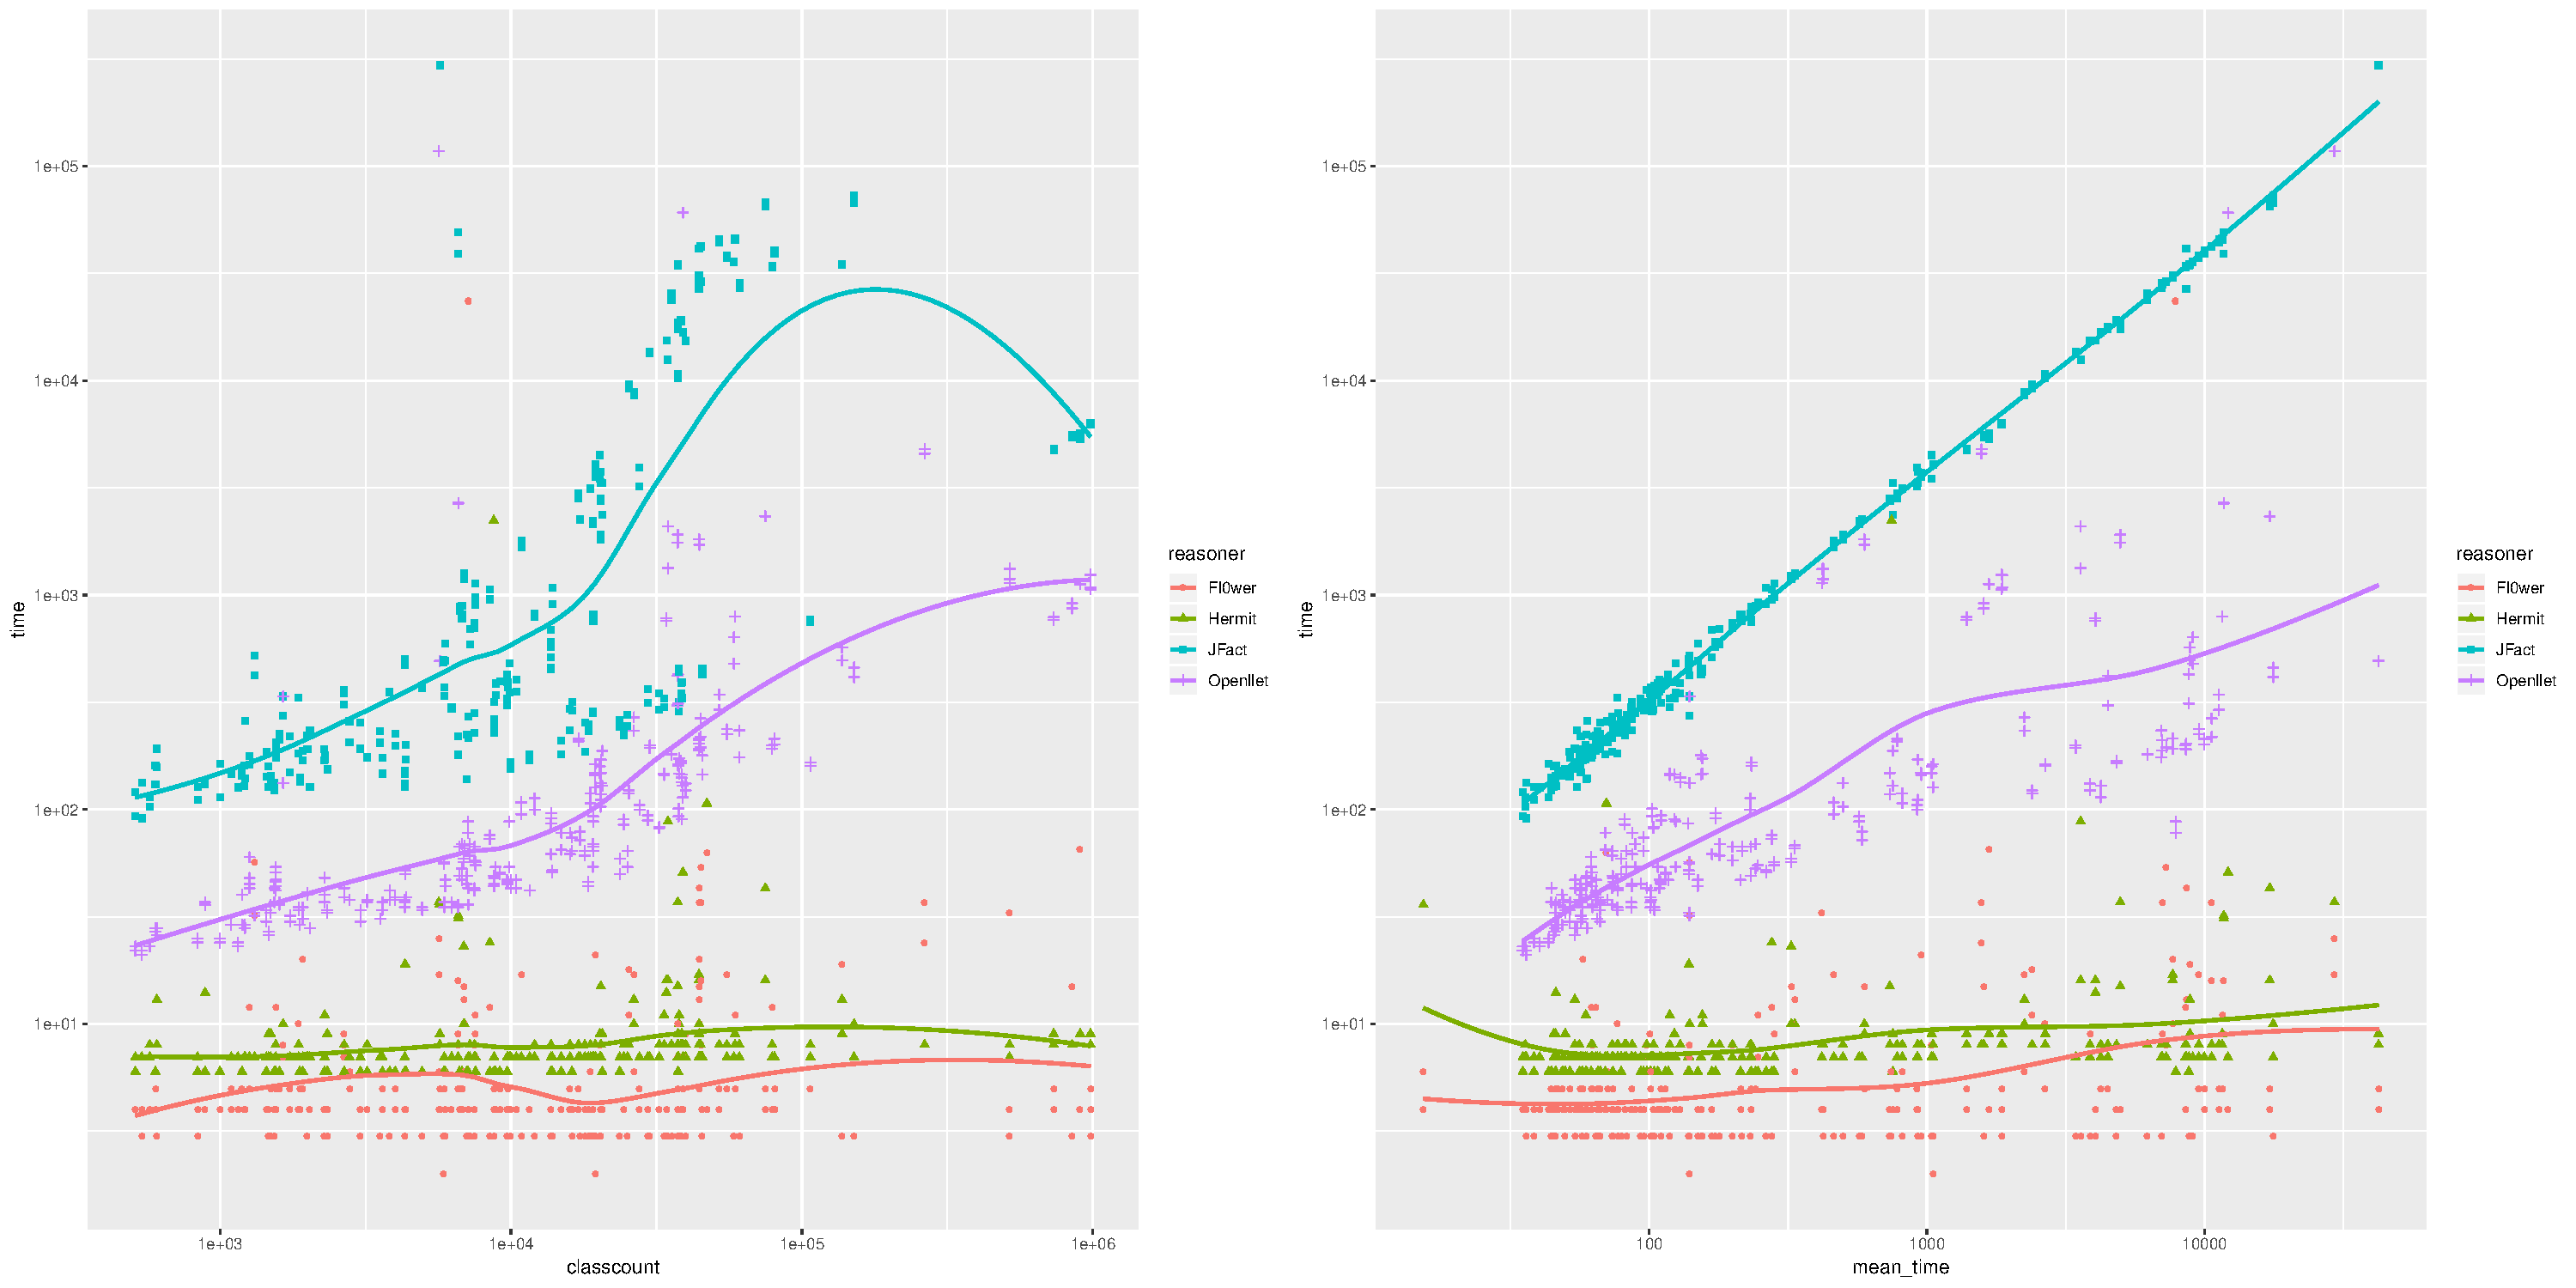
\includegraphics[width=15cm]{fig/subsumption.pdf}
	\caption{Subsumption}
	\label{fig2}
\end{figure}

\begin{figure}[ht]
	\centering
	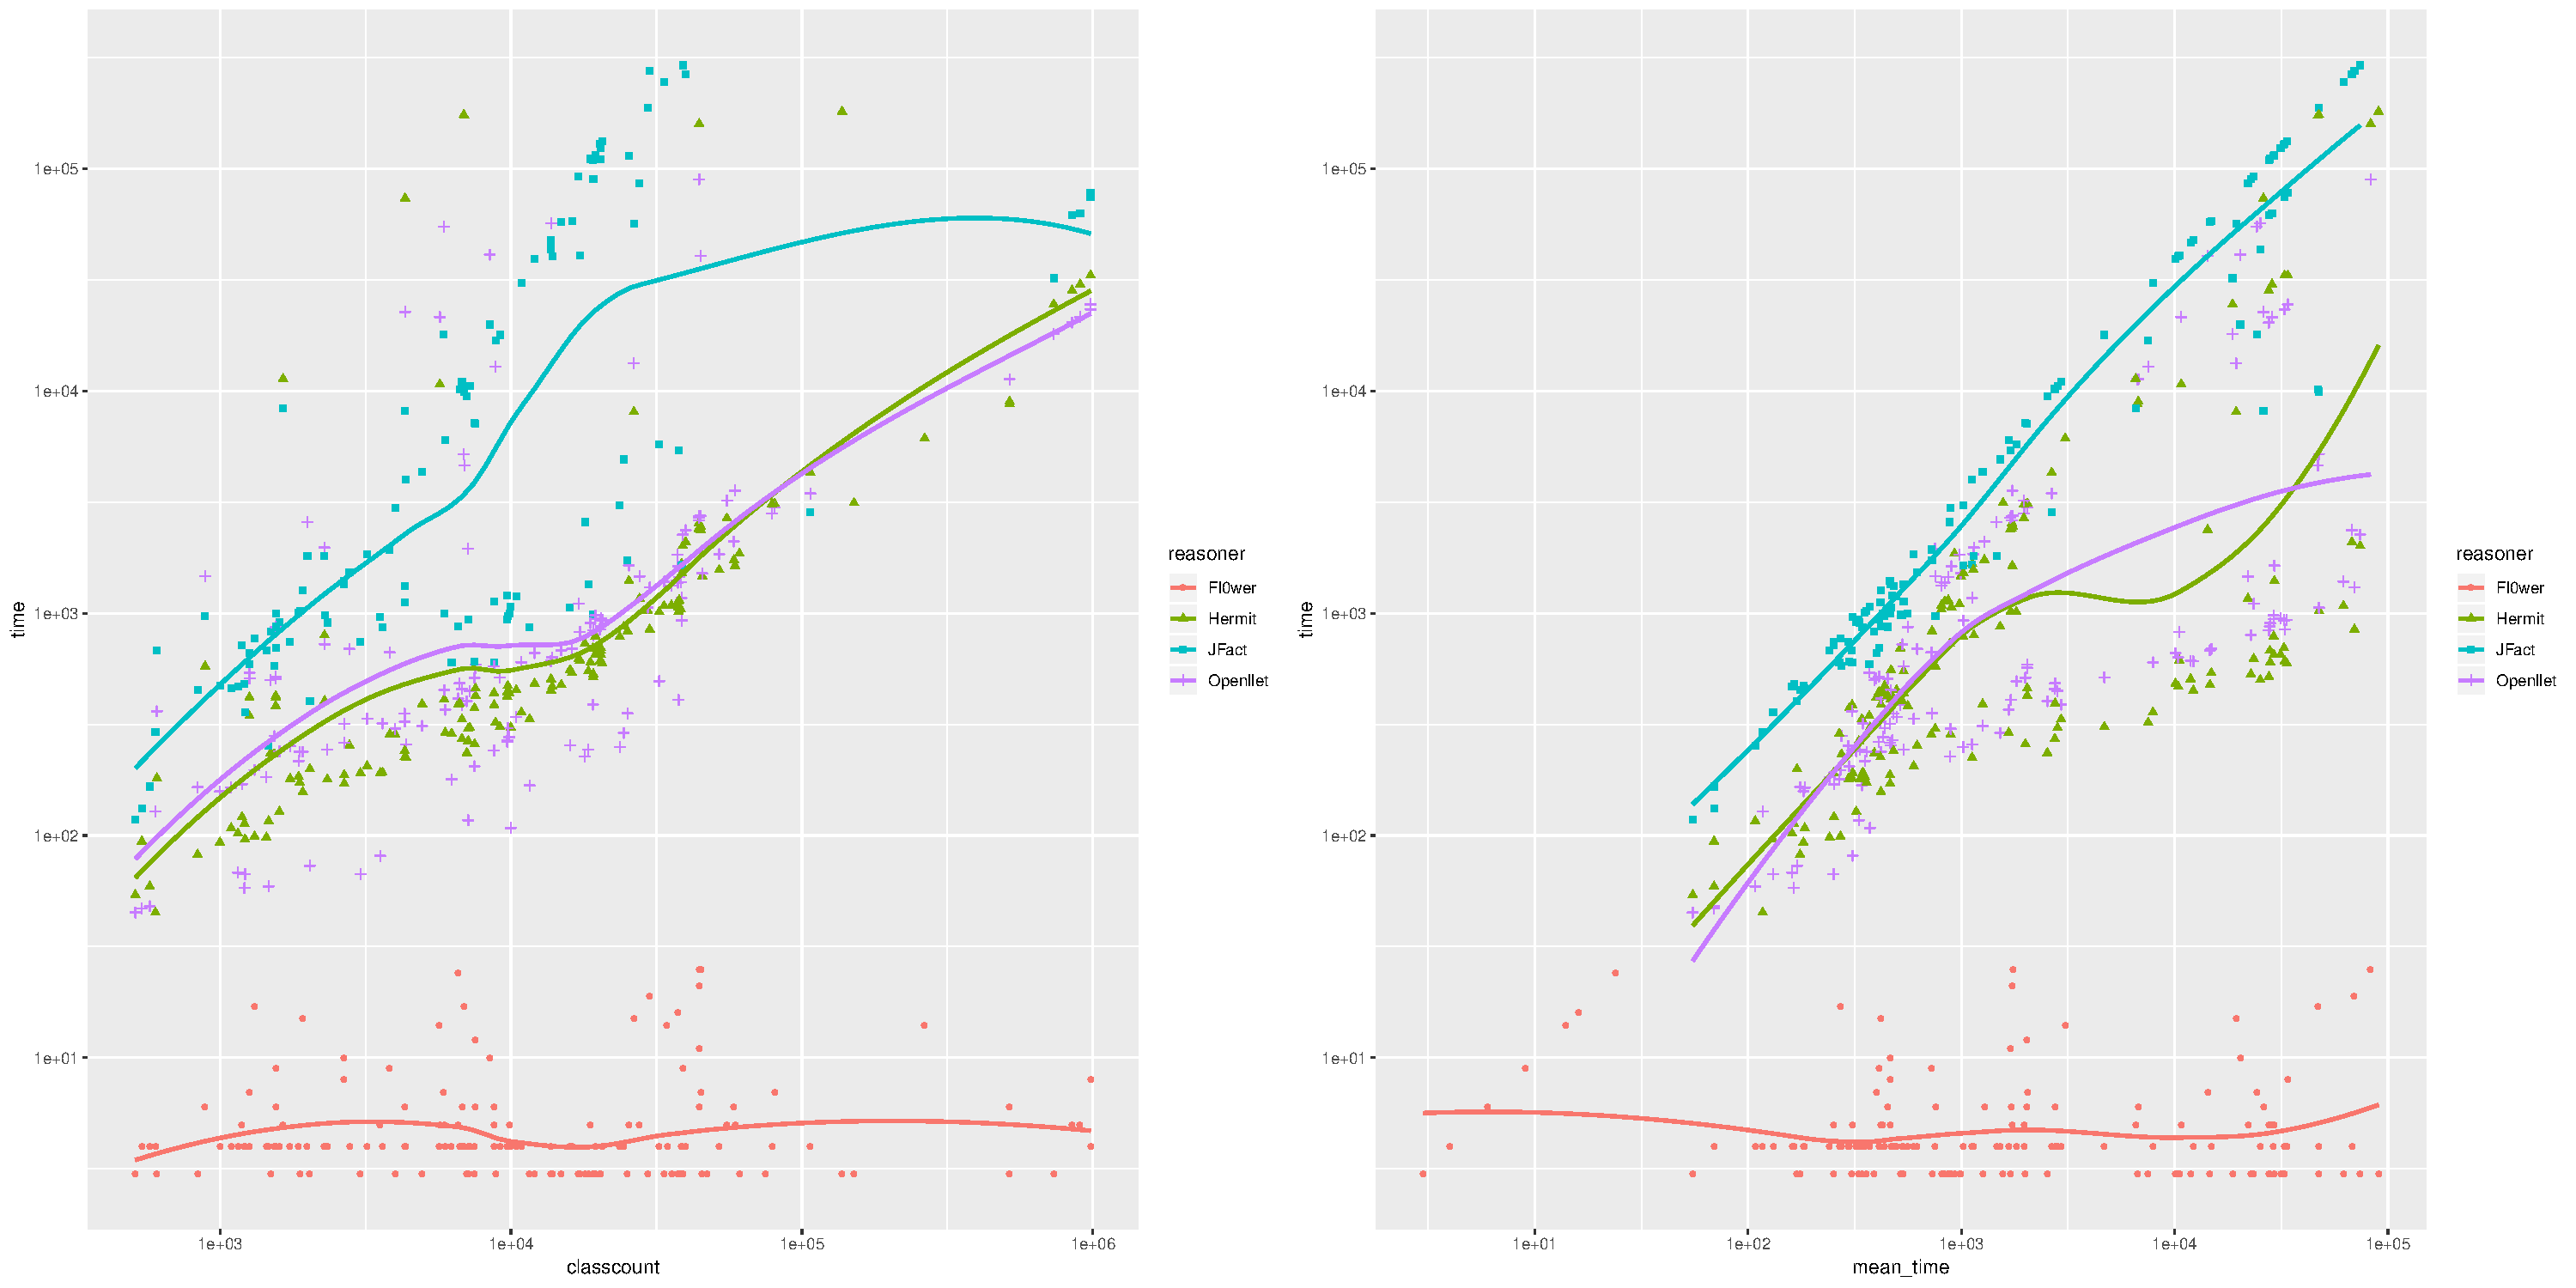
\includegraphics[width=15cm]{fig/subsumerset.pdf}
	\caption{Subsumerset}
	\label{fig2}
\end{figure}

\begin{figure}[ht]
	\centering
	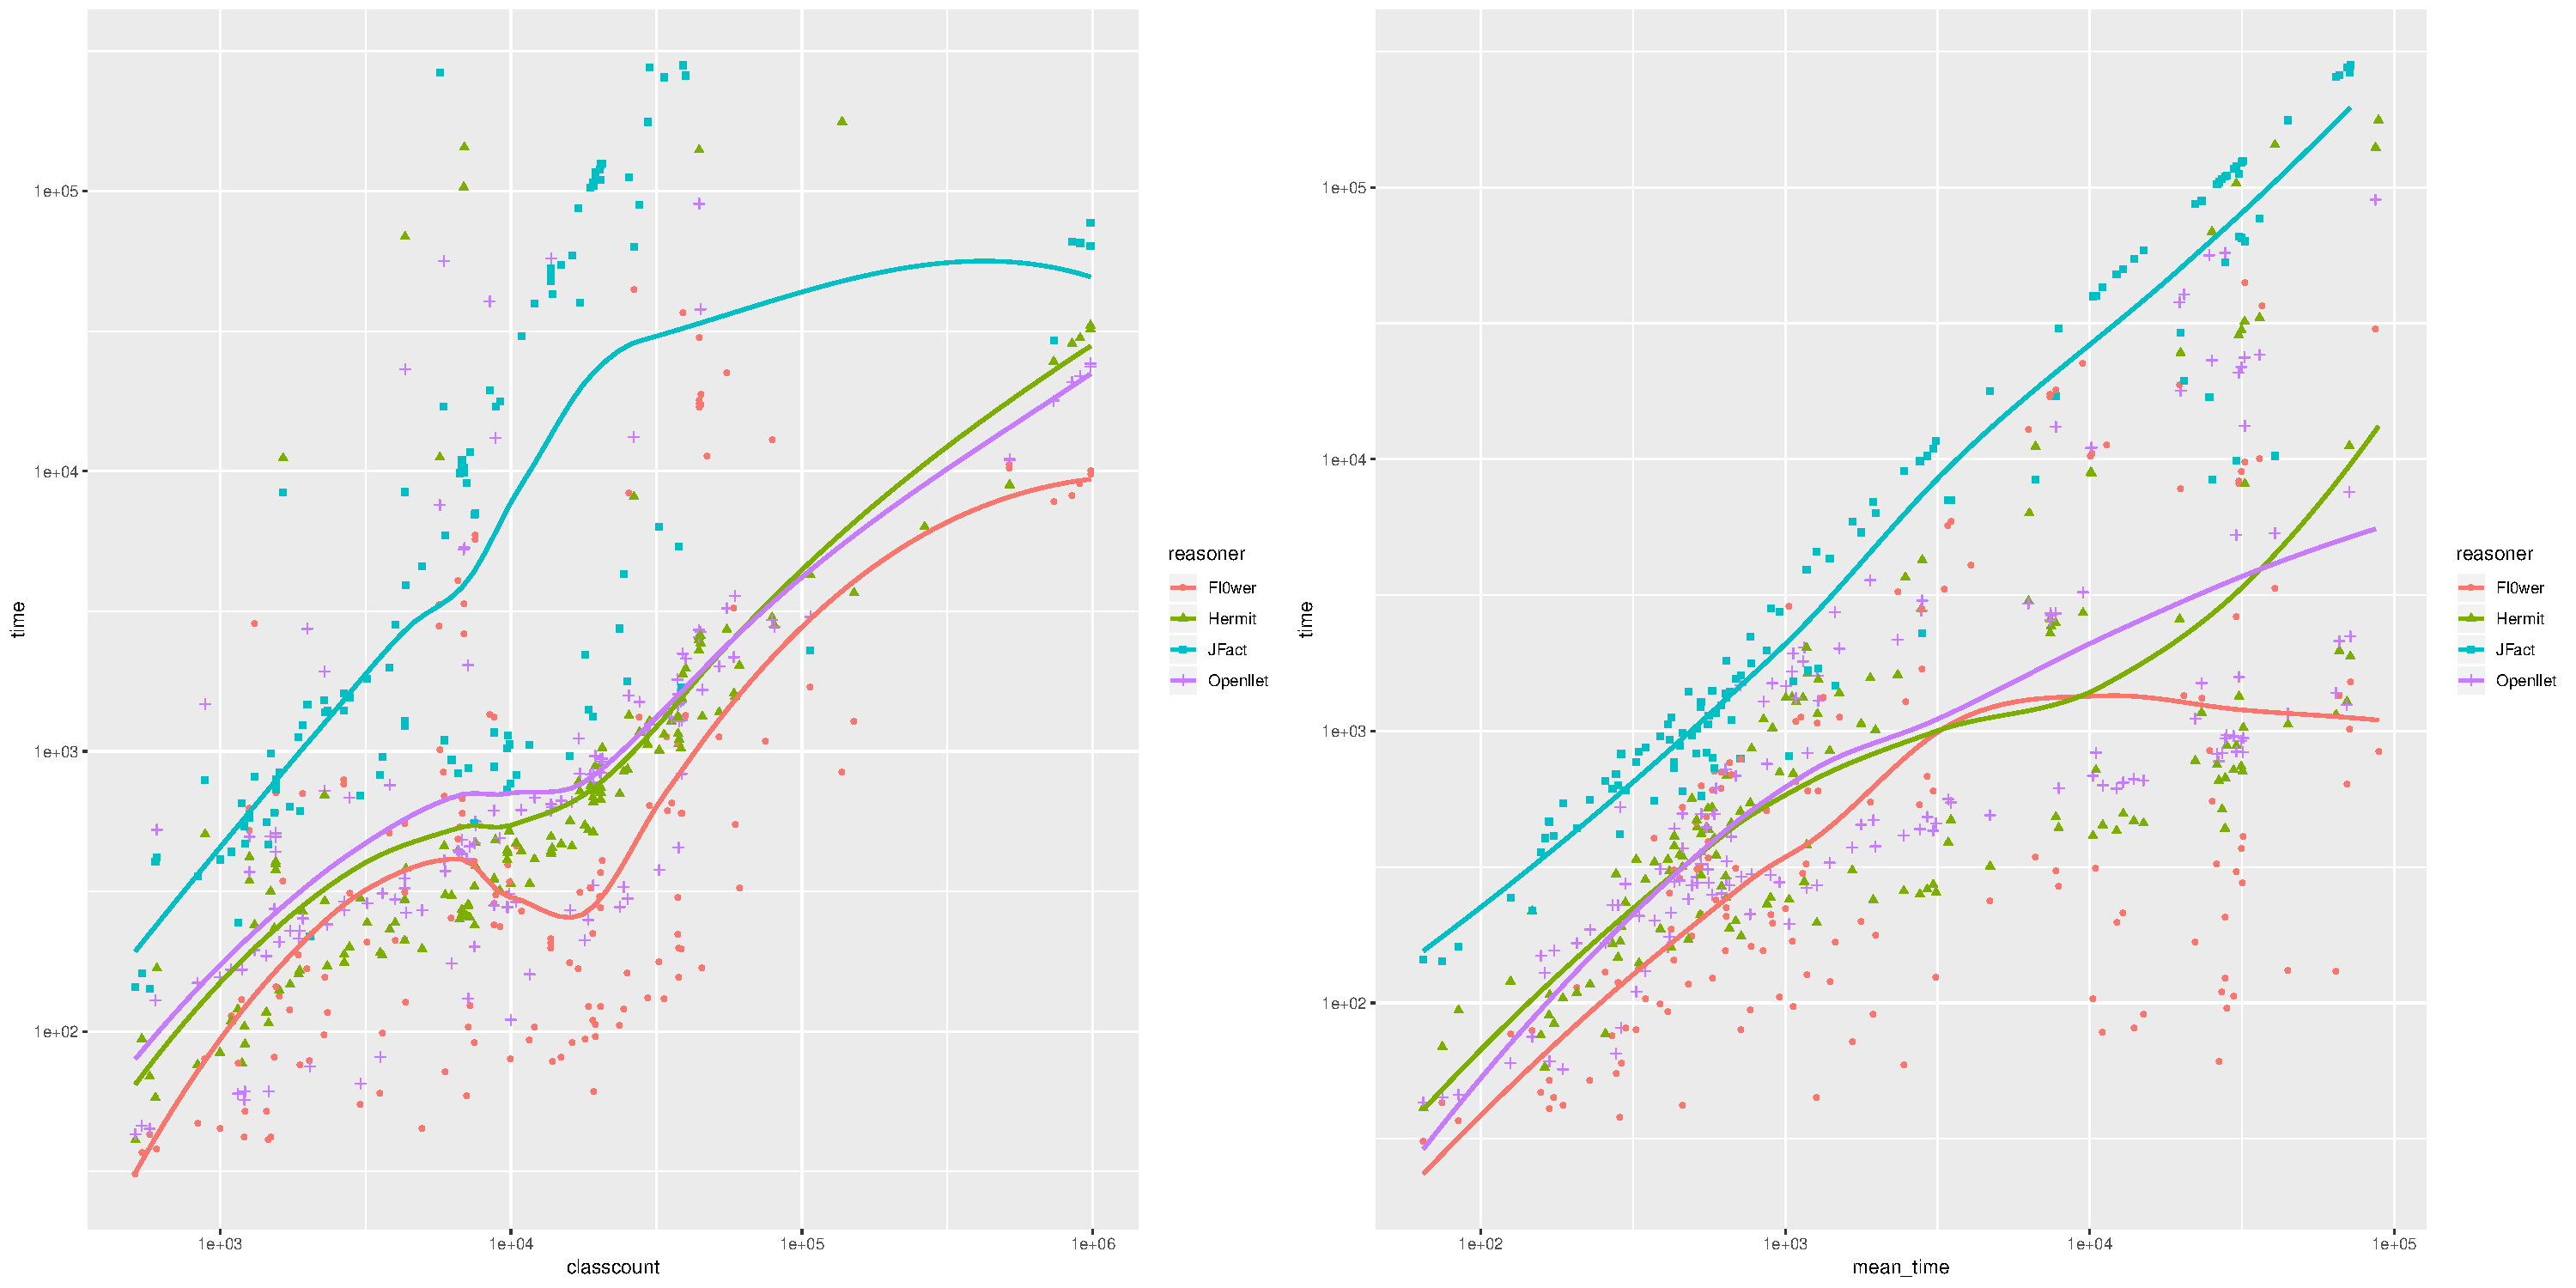
\includegraphics[width=15cm]{fig/classification.pdf}
	\caption{Classification}
	\label{fig2}
\end{figure}


\bibliographystyle{unsrt}
\bibliography{bibliography}

\end{document}
